\documentclass[11pt,a4paper]{article}
\usepackage[margin=2.1cm]{geometry}
\usepackage{amsmath,amssymb}
\usepackage{enumitem}
\usepackage{fancyhdr}
\usepackage{booktabs}
\usepackage{array}
\usepackage{graphicx}
\usepackage{tikz}
\usetikzlibrary{positioning,arrows.meta,calc}
\usepackage[most]{tcolorbox}
\usepackage{kotex}
\setmainhangulfont{Nanum Myeongjo}
\setsanshangulfont{Apple SD Gothic Neo}
\usepackage[hidelinks]{hyperref}

\pagestyle{fancy}
\fancyhf{}
\lhead{Classification Workbook}
\rhead{코드로 연습하는 분류}
\cfoot{\thepage}
\setlength{\headheight}{14pt}
\setlength{\parindent}{0pt}
\setlength{\parskip}{0.45em}
\setlength{\emergencystretch}{2em}
\setlist[itemize]{leftmargin=1.3em,itemsep=0.2em,topsep=0.2em}
\setlist[enumerate]{leftmargin=1.6em,itemsep=0.2em,topsep=0.2em}
\renewcommand{\arraystretch}{1.15}
\AddToHook{cmd/section/before}{\clearpage}
\sloppy

\newcommand{\term}[1]{\textbf{#1}}
\newcommand{\code}[1]{\texttt{#1}}
\newcommand{\aside}[1]{{\footnotesize\color{black!65}#1}}
\newcommand{\Ans}{\par\textbf{Answer.}\ }

\newtcolorbox{codebox}[1][]{breakable,colback=black!3,colframe=black!45,boxrule=0.5pt,arc=1.5pt,
  left=4pt,right=4pt,top=2pt,bottom=2pt,fontupper=\small\ttfamily,#1}
\newtcolorbox{outbox}{breakable,colback=green!3,colframe=green!35!black,boxrule=0.5pt,arc=1.5pt,
  left=4pt,right=4pt,top=2pt,bottom=2pt,fontupper=\small\ttfamily,
  fonttitle=\bfseries\sffamily\small,title={실행 결과}}
\newtcolorbox{goalbox}[1]{colback=blue!4,colframe=blue!45!black,boxrule=0.6pt,arc=1.5pt,
  fonttitle=\bfseries\sffamily,title={#1}}
\newtcolorbox{howbox}{breakable,colback=orange!4,colframe=orange!60!black,boxrule=0.6pt,arc=1.5pt,
  fonttitle=\bfseries\sffamily,title={무슨 일이 일어났나}}
\newtcolorbox{qbox}{breakable,colback=gray!5,colframe=gray!55!black,boxrule=0.5pt,arc=1.5pt,
  fonttitle=\bfseries\sffamily\small,title={확인 질문}}

% 다이어그램 노드 스타일
\tikzset{
  wstep/.style={draw, rounded corners=3pt, minimum width=3.6cm, minimum height=1.55cm,
    align=center, font=\small, line width=0.6pt},
  prep/.style={wstep, fill=blue!7, draw=blue!50!black},
  model/.style={wstep, fill=orange!8, draw=orange!65!black},
  check/.style={wstep, fill=green!7, draw=green!45!black},
  arr/.style={-{Stealth[length=2.6mm]}, line width=0.8pt, black!70},
}
\newcommand{\nd}[3]{\textbf{#1}\\[-1pt]{\footnotesize #2}\\[-1pt]{\scriptsize\ttfamily\color{black!70}#3}}

\begin{document}

%================= 첫 페이지: 제목 + 전체 흐름 다이어그램 =================
\thispagestyle{empty}
\begin{center}
{\LARGE\textbf{코드로 연습하는 분류 (Classification)}}\\[0.35em]
{\large 채용 데이터로 ``합격 여부''를 예측하며 배우는 머신러닝의 전 과정}\\[0.25em]
{\small 연습 노트북: \code{classification\_practice.ipynb} (빈칸) \quad 정답: \code{classification\_solution.ipynb}}
\end{center}

\vspace{0.6em}
\begin{center}
\begin{tikzpicture}[node distance=0.55cm and 0.55cm]
% 1행: 준비
\node[prep] (s1) {\nd{① 문제 정의}{무엇을 예측? 왜?}{1장}};
\node[prep, right=of s1] (s2) {\nd{② 데이터 준비}{X(설명) / y(정답)}{2장 · Step 1}};
\node[prep, right=of s2] (s3) {\nd{③ 나누기}{train 75\% / test 25\%}{3장 · Step 2}};
\node[prep, right=of s3] (s4) {\nd{④ 기준선}{찍기만 해도 몇 점?}{4장 · Step 3}};
% 2행: 모델링 (오른쪽에서 왼쪽)
\node[model, below=1.3cm of s4] (s5) {\nd{⑤ 전처리}{범주$\to$0/1, 숫자$\to$표준화}{5장 · Step 4}};
\node[model, left=of s5] (s6) {\nd{⑥ 학습·예측}{fit $\to$ predict\_proba}{6장 · Step 5}};
\node[model, left=of s6] (s7) {\nd{⑦ 평가}{혼동행렬, 정밀도, 재현율}{7장 · Step 6}};
\node[model, left=of s7] (s8) {\nd{⑧ 임계값·ROC}{0.5가 최선인가? AUC}{8장 · Step 7}};
% 3행: 검증과 해석
\node[check, below=1.6cm of s8] (s9) {\nd{⑨ 모델 비교}{tree, forest, 교차검증}{9장 · Step 8}};
\node[check, right=of s9] (s10) {\nd{⑩ 해석}{odds ratio, 중요도}{10장 · Step 9}};
\node[check, right=of s10] (s11) {\nd{⑪ 공정성 감사}{그룹별 TPR, 성별 제거}{11장 · Step 10}};
\node[check, right=of s11] (s12) {\nd{⑫ 결론·발표}{무엇을 말할 수 있나}{12장}};
% 화살표
\draw[arr] (s1) -- (s2); \draw[arr] (s2) -- (s3); \draw[arr] (s3) -- (s4);
\draw[arr] (s4) -- (s5);
\draw[arr] (s5) -- (s6); \draw[arr] (s6) -- (s7); \draw[arr] (s7) -- (s8);
\draw[arr] (s8) -- (s9);
\draw[arr] (s9) -- (s10); \draw[arr] (s10) -- (s11); \draw[arr] (s11) -- (s12);
% 개선 반복 루프: 평가 -> 전처리
\draw[arr, dashed, red!65!black] (s7.south) to[bend right=22] node[below, font=\scriptsize, text=red!65!black, fill=white, inner sep=1pt] {개선 반복 (특성·모델 바꾸기)} (s5.south);
% test set은 마지막 평가에만: 나누기 -> 평가
\draw[arr, dotted, blue!60!black] (s3.south) .. controls +(0,-0.6) and +(0,0.9) .. node[pos=0.55, fill=white, font=\scriptsize, text=blue!60!black, inner sep=1pt] {test는 평가에만} (s7.north east);
\end{tikzpicture}
\end{center}

\vspace{0.3em}
\begin{center}\small
\begin{tabular}{@{}c l l@{}}
\tikz\node[prep, minimum width=0.5cm, minimum height=0.35cm]{}; & \textbf{준비} (①–④) & 데이터를 모델이 먹을 수 있게, 그리고 공정하게 평가할 수 있게 \\
\tikz\node[model, minimum width=0.5cm, minimum height=0.35cm]{}; & \textbf{모델링} (⑤–⑧) & 학습하고, 예측하고, 얼마나 맞는지 잰다 \\
\tikz\node[check, minimum width=0.5cm, minimum height=0.35cm]{}; & \textbf{검증·해석} (⑨–⑫) & 다른 모델과 비교하고, 이유와 공정성을 따진다 \\
\end{tabular}
\end{center}

\begin{goalbox}{이 워크북의 핵심 메시지}
채용 데이터로 합격 예측 모델을 만들면 모델은 \emph{과거 채용의 편향까지} 배웁니다. 그래서 이 워크북의 목표는 ``좋은 채용 AI 만들기''가 아니라, \textbf{분류 모델을 만들어 보면서 그 모델이 어떤 편향을 재생산하는지 감사(audit)하는 것}입니다. 이것이 datathon 주제 ``Exploring Bias in Hiring''과 연결되는 지점입니다.
\end{goalbox}

\clearpage
\renewcommand{\contentsname}{목차 (Contents)}
\tableofcontents

%=================================================
\section*{0\quad 이 워크북 쓰는 법}
\addcontentsline{toc}{section}{0\quad 이 워크북 쓰는 법}

\subsection*{준비물}
\begin{itemize}
\item 폴더 \code{\textasciitilde/DataPythonPrep}: \code{hiring\_practice.csv}, \code{classification\_practice.ipynb} (빈칸), \code{classification\_solution.ipynb} (정답, 실행 결과 포함).
\item VS Code나 Jupyter에서 \code{classification\_practice.ipynb}를 엽니다.
\end{itemize}
\begin{codebox}
cd \textasciitilde/DataPythonPrep\\
jupyter notebook classification\_practice.ipynb \hfill \# 또는 VS Code에서 열기
\end{codebox}

\subsection*{각 장의 구성}
\begin{center}\small
\begin{tabular}{@{}l l@{}}
\toprule
상자 & 하는 일 \\
\midrule
\textcolor{blue!45!black}{\textbf{목표}} & 이 단계에서 할 일 한 줄, 다이어그램의 위치 \\
본문 & 필요한 개념만 짧게 \\
\textbf{코드 (빈칸)} & 노트북과 같은 코드. \code{\_\_\_}를 채워서 실행 \\
\textcolor{green!35!black}{\textbf{실행 결과}} & 실제로 돌린 출력. 내 결과와 비교 \\
\textcolor{orange!60!black}{\textbf{무슨 일이 일어났나}} & 코드가 데이터를 어떻게 바꿨는지 단계별로 \\
\textbf{확인 질문} & 이해했는지 점검 (답은 13장) \\
\bottomrule
\end{tabular}
\end{center}
\aside{※ 빈칸 정답은 13장 끝 ``빈칸 정답''과 정답 노트북에 있습니다. 막히면 5분 고민 후 보세요.}\\
\aside{※ 다른 책과의 연결: [흐름 $n$] = pandas-stats-walkthrough, [응용 $n$] = hiring-statistics-book, [알고 $n$] = algorithms-for-datathon.}

\subsection*{회귀 분석(다른 책)과 무엇이 다른가}
\begin{center}\small
\begin{tabular}{@{}l l l@{}}
\toprule
 & 통계 회귀 (응용 책) & 분류 머신러닝 (이 책) \\
\midrule
목적 & \textbf{설명}: 성별 효과가 몇 \%p인가, 유의한가 & \textbf{예측}: 새 지원자가 합격할까 \\
데이터 사용 & 전부로 추정 & train으로 학습, test로 평가 \\
성공 기준 & p-value, 신뢰구간 & 정확도, 정밀도, 재현율, AUC \\
도구 & \code{statsmodels} & \code{scikit-learn} \\
\bottomrule
\end{tabular}
\end{center}
같은 logistic regression이 두 책에 다 나오지만, 묻는 질문이 다릅니다.

%=================================================
\section{분류란 무엇인가: 문제 정의}
\begin{goalbox}{목표 \quad ①}
``무엇을, 무엇으로, 왜 예측하는가''를 한 문장으로 정한다.
\end{goalbox}

\subsection{분류 (classification)}
정답이 \textbf{범주}인 예측 문제입니다. 정답이 숫자면 \term{regression}(회귀)입니다.
\begin{center}\small
\begin{tabular}{@{}l l l@{}}
\toprule
예 & 정답 $y$ & 종류 \\
\midrule
이 지원자가 합격할까 & 0 / 1 & \textbf{이진 분류} (binary) \\
이 메일은 스팸일까 & 0 / 1 & 이진 분류 \\
어느 부서에 맞을까 & Engineering / Marketing / \dots & 다중 분류 (multiclass) \\
시험 점수는 몇 점일까 & 29–100 숫자 & 회귀 \\
\bottomrule
\end{tabular}
\end{center}

\subsection{이번 문제}
\begin{itemize}
\item \textbf{정답 $y$}: \code{hired} (1 = 합격, 0 = 불합격)
\item \textbf{설명변수 $X$}: \code{gender}, \code{department}, \code{degree}, \code{test\_score}, \code{years\_experience}
\item \textbf{학습이란}: $X$와 $y$의 짝 수백 개를 보고, $X$만 주면 $y$를 맞히는 규칙 $f$를 찾는 것: $\hat y=f(X)$.
\end{itemize}

\subsection{먼저 생각할 것: 이 모델을 왜 만드나}
\begin{itemize}
\item 과거 채용 결과($y$)가 편향되어 있으면, 그것을 잘 맞히는 모델은 \textbf{편향을 잘 배운 모델}입니다. 정확도가 높을수록 공정하다는 뜻이 아닙니다.
\item 그래서 이 문제의 올바른 사용법은 (1) 어떤 특성이 결과를 좌우하는지 이해하고, (2) 모델이 그룹별로 다르게 틀리는지 감사하는 것입니다 (11장).
\end{itemize}
\aside{※ 실제 사례: 2018년 한 대형 기업이 이력서 평가 모델을 폐기했습니다. 과거 채용 데이터가 남성 위주라서 모델이 ``여성''과 관련된 단어에 감점을 학습했기 때문입니다.}

\begin{qbox}
1. ``지원자의 예상 연봉 맞히기''는 분류인가 회귀인가?\quad
2. 테스트 정확도 95\%인 채용 모델은 공정하다고 할 수 있는가?
\end{qbox}

%=================================================
\section{Step 1. 데이터 준비: X와 y}
\begin{goalbox}{목표 \quad ②}
표에서 \textbf{문제지(X)}와 \textbf{정답지(y)}를 분리한다.
\end{goalbox}

\begin{codebox}
df = pd.read\_csv("hiring\_practice.csv")\\
d = df.\_\_\_() \hfill \# 결측 행 제거\\
cat = ["gender", "department", "degree"] \hfill \# 범주형 열\\
num = ["test\_score", "years\_experience"] \hfill \# 숫자형 열\\
X = d[\_\_\_] \hfill \# 설명변수 5개\\
y = d[\_\_\_] \hfill \# 결과변수\\
print(X.shape, round(y.mean(), 3))
\end{codebox}
\begin{outbox}
(582, 5) 0.325
\end{outbox}

\begin{howbox}
\begin{enumerate}
\item \code{dropna()}: \code{test\_score}가 빈 18행을 지워 600 $\to$ 582행. (모델은 \code{NaN}을 받지 못합니다.)
\item \code{X = d[cat + num]}: 리스트 두 개를 이어 붙인 5개 열만 고른 DataFrame. \code{applicant\_id}와 \code{hired}는 빠집니다.
\item \code{y = d["hired"]}: 열 하나 = Series.
\item \code{y.mean()} = 0.325: 582명 중 32.5\%가 합격. 이 숫자가 4장 기준선의 출발점입니다.
\end{enumerate}
\end{howbox}
\aside{※ \code{applicant\_id}를 X에 넣으면 안 됩니다. 번호에는 의미가 없는데, 모델은 우연한 패턴을 배울 수 있습니다. [응용 2.2]}\\
\aside{※ 정답 열(\code{hired})이나 정답에서 파생된 열이 X에 섞이면 \term{data leakage}: 테스트 점수가 비현실적으로 높게 나옵니다.}

\begin{qbox}
3. \code{X = d.drop(columns=["applicant\_id", "hired"])}는 위 코드와 같은 결과인가?
\end{qbox}

%=================================================
\section{Step 2. train / test 나누기}
\begin{goalbox}{목표 \quad ③}
모델이 \textbf{본 적 없는} 데이터로 평가할 수 있도록 일부를 떼어 둔다.
\end{goalbox}

\subsection{왜 나누나: 과적합 (overfitting)}
시험 문제를 미리 보고 공부하면 그 시험은 100점이지만 실력은 모릅니다. 모델도 학습에 쓴 데이터로 평가하면 \textbf{외운 것}과 \textbf{배운 것}을 구분할 수 없습니다.
\begin{itemize}
\item \term{Training set}: 모델이 규칙을 배우는 데이터 (75\%)
\item \term{Test set}: 마지막에 한 번, 성적표를 받는 데이터 (25\%). \textbf{학습·튜닝에 절대 쓰지 않습니다.}
\end{itemize}

\begin{codebox}
X\_train, X\_test, y\_train, y\_test = train\_test\_split(\\
\ \ \ \ X, y, test\_size=\_\_\_, stratify=\_\_\_, random\_state=0)\\
print(len(X\_train), len(X\_test), round(y\_train.mean(), 3), round(y\_test.mean(), 3))
\end{codebox}
\begin{outbox}
436 146 0.326 0.322
\end{outbox}

\begin{howbox}
\begin{enumerate}
\item 582행의 순서를 무작위로 섞습니다 (\code{random\_state=0}: 매번 같은 섞기 $\to$ 결과 재현 가능).
\item 25\% = 146행을 test로, 나머지 436행을 train으로.
\item \code{stratify=y}: 합격자 비율(32.5\%)이 양쪽에서 같도록 \emph{합격자/불합격자 각각} 25\%씩 떼어 냅니다. 그래서 0.326과 0.322로 거의 같습니다.
\item 결과는 4개: 문제지와 정답지가 각각 train/test로.
\end{enumerate}
\end{howbox}
\aside{※ 통계 연결: test 점수도 146명 표본에서 나온 \emph{추정값}이라 흔들립니다. 그래서 9장에서 교차검증으로 여러 번 잽니다. [흐름 4, 9]}

\begin{qbox}
4. \code{stratify}를 빼면 어떤 문제가 생길 수 있나? 특히 합격자가 5\%뿐인 데이터라면?
\end{qbox}

%=================================================
\section{Step 3. 기준선 (baseline)}
\begin{goalbox}{목표 \quad ④}
``아무 생각 없이 찍어도'' 받는 점수를 먼저 안다. 모델은 이것보다 나아야 의미가 있다.
\end{goalbox}

\begin{codebox}
dummy = DummyClassifier(strategy=\_\_\_).fit(X\_train, y\_train)\\
print(round(accuracy\_score(y\_test, dummy.predict(X\_test)), 3))
\end{codebox}
\begin{outbox}
0.678
\end{outbox}

\begin{howbox}
\begin{enumerate}
\item \code{"most\_frequent"}: train에서 가장 많은 답 (불합격 = 0)을 찾습니다.
\item test 146명 \emph{모두에게} 0이라고 예측합니다. X는 보지도 않습니다.
\item test의 실제 불합격자 99명을 다 맞히므로 정확도 $99/146=0.678$.
\end{enumerate}
\end{howbox}
\textbf{교훈}: 정확도 68\%는 ``아무것도 안 배운'' 점수입니다. 불균형 데이터에서 정확도만 보면 속습니다. 이 모델은 합격자를 \emph{한 명도} 찾지 못합니다 (재현율 0). 그래서 7장의 다른 지표가 필요합니다.

\begin{qbox}
5. 합격률이 5\%인 데이터에서 ``전원 불합격'' 모델의 정확도는?
\end{qbox}

%=================================================
\section{Step 4. 전처리 파이프라인}
\begin{goalbox}{목표 \quad ⑤}
문자열과 크기가 다른 숫자를, 모델이 계산할 수 있는 \textbf{숫자 행렬}로 바꾼다.
\end{goalbox}

\subsection{두 가지 변환}
\begin{itemize}
\item \term{One-hot encoding}: \code{"Marketing"} $\to$ \code{department\_Marketing = 1}. \code{drop="first"}는 기준 범주 열을 빼서 중복을 없앱니다 (응용 책의 dummy와 같음 [응용 0.8, 6.4]).
\item \term{Standardization}: $z=(x-\bar x)/\text{SD}$. 점수(29–100)와 경력(0–11)의 단위를 맞춥니다 [흐름 3.1]. logistic의 규제(regularization)는 계수 크기에 벌점을 주므로 단위가 같아야 공평합니다.
\end{itemize}

\begin{codebox}
pre = ColumnTransformer([\\
\ \ \ \ ("cat", \_\_\_(drop="first"), cat), \hfill \# 범주 $\to$ 0/1 열\\
\ \ \ \ ("num", \_\_\_(), num), \hfill \# 숫자 $\to$ 평균 0, SD 1\\
])\\
pre.fit(X\_train)\\
print(pre.get\_feature\_names\_out())\\
print(pre.transform(X\_train.head(3)).round(2))
\end{codebox}
\begin{outbox}
['cat\_\_gender\_M' 'cat\_\_department\_Marketing' 'cat\_\_degree\_Master'\\
\ 'cat\_\_degree\_PhD' 'num\_\_test\_score' 'num\_\_years\_experience']\\
{}[[ 1.\ \ \ 0.\ \ \ 1.\ \ \ 0.\ \ -0.81 -0.78]\\
\ [ 0.\ \ \ 1.\ \ \ 0.\ \ \ 0.\ \ \ 0.73\ \ 1.76]\\
\ [ 1.\ \ \ 0.\ \ \ 0.\ \ \ 0.\ \ -0.04 -1.29]]
\end{outbox}

\begin{howbox}
train 첫 행 (M, Engineering, Master, 56점, 3년)이 어떻게 바뀌었나:
\begin{center}\small
\begin{tabular}{@{}l l r@{}}
\toprule
원래 값 & 변환 & 결과 \\
\midrule
gender = M & one-hot & \code{gender\_M} = 1 \\
department = Engineering & 기준 범주 & \code{department\_Marketing} = 0 \\
degree = Master & one-hot & \code{Master} = 1, \code{PhD} = 0 \\
test\_score = 56 & $(56-65.49)/11.66$ & $-0.81$ \\
years\_experience = 3 & $(3-4.53)/1.97$ & $-0.78$ \\
\bottomrule
\end{tabular}
\end{center}
평균 65.49와 SD 11.66은 \textbf{train에서만} 계산한 값입니다 (\code{pre.fit(X\_train)}). test에는 같은 숫자를 그대로 적용합니다.
\end{howbox}
\aside{※ test의 평균으로 표준화하면 test 정보가 학습에 새어 들어갑니다 (leakage). \code{Pipeline}에 넣으면 이 순서가 자동으로 지켜집니다.}

\begin{qbox}
6. 표준화 없이 logistic regression을 돌리면 \code{test\_score} 계수의 단위는 무엇인가?
\end{qbox}

%=================================================
\section{Step 5. 학습과 예측}
\begin{goalbox}{목표 \quad ⑥}
logistic regression을 학습시키고, test 지원자마다 \textbf{합격 확률}과 \textbf{0/1 예측}을 얻는다.
\end{goalbox}

\subsection{모델}
\[
P(\text{hired}=1\mid x)=\sigma(b_0+b_1x_1+\dots+b_6x_6),\qquad \sigma(z)=\frac1{1+e^{-z}}.
\]
\code{fit}은 train 436명의 likelihood를 최대화하는 $b$를 찾습니다 (MLE, Newton류 반복) [응용 7.2]. 그다음 확률이 임계값(기본 0.5) 이상이면 1로 예측합니다.

\begin{codebox}
logit = Pipeline([("pre", pre), ("clf", LogisticRegression(max\_iter=1000))])\\
logit.\_\_\_(X\_train, y\_train)\\
p = logit.\_\_\_(X\_test)[:, 1] \hfill \# 합격 확률 (두 번째 열)\\
y\_hat = (p >= \_\_\_).astype(int)\\
print(p[:5].round(3), y\_hat[:5])
\end{codebox}
\begin{outbox}
[0.502 0.286 0.535 0.091 0.427] [1 0 1 0 0]
\end{outbox}

\begin{howbox}
\begin{enumerate}
\item \code{fit}: 파이프라인이 \code{pre.fit\_transform(X\_train)} $\to$ \code{clf.fit(행렬, y\_train)} 순서로 실행.
\item \code{predict\_proba(X\_test)}: \code{pre.transform}(train의 평균/SD 사용) $\to$ 확률. 결과는 146$\times$2 배열 (열 0 = 불합격 확률, 열 1 = 합격 확률). \code{[:, 1]}로 합격 쪽만.
\item test 첫 번째 지원자 (M, Engineering, Master, 73점, 3년, 실제 합격)의 계산:
\[
z=\underbrace{-0.596}_{b_0}+\underbrace{0.297}_{\text{M}}+\underbrace{0.175}_{\text{Master}}+\underbrace{0.627\times0.644}_{\text{점수 }z=0.644}+\underbrace{0.351\times(-0.779)}_{\text{경력 }z=-0.779}=0.008,
\]
$\sigma(0.008)=0.502\ \Rightarrow$ 0.5 이상이라 \textbf{합격(1)} 예측. 맞았습니다.
\item 다섯 번째 (M, Engineering, Master, 74점, 1년, 실제 합격): 0.427 $\Rightarrow$ 불합격 예측. 틀렸습니다 (경력이 짧아서).
\end{enumerate}
\end{howbox}

\begin{qbox}
7. 위 계산에서 \code{department\_Marketing} 항이 0인 이유는?
\end{qbox}

%=================================================
\section{Step 6. 평가: 혼동행렬과 지표}
\begin{goalbox}{목표 \quad ⑦}
146명에 대한 예측을 \textbf{네 칸}으로 나누고, 목적에 맞는 점수를 계산한다.
\end{goalbox}

\subsection{혼동행렬 (confusion matrix)}
\begin{center}
\begin{tabular}{@{}l c c@{}}
\toprule
 & 예측 0 (불합격) & 예측 1 (합격) \\
\midrule
실제 0 & \textbf{TN} = 95 \ (맞게 거절) & \textbf{FP} = 4 \ (잘못 합격) \\
실제 1 & \textbf{FN} = 31 \ (놓침) & \textbf{TP} = 16 \ (맞게 합격) \\
\bottomrule
\end{tabular}
\end{center}
\aside{※ sklearn의 출력 \code{[[95 4] [31 16]]}은 위 표와 같은 배치입니다: 행 = 실제, 열 = 예측.}

\subsection{지표}
\begin{center}\small
\begin{tabular}{@{}l l l r@{}}
\toprule
지표 & 식 & 질문 & 값 \\
\midrule
\term{Accuracy} & $\frac{TP+TN}{\text{전체}}$ & 전체 중 몇 \% 맞혔나 & $\frac{111}{146}=0.760$ \\
\term{Precision} & $\frac{TP}{TP+FP}$ & 합격이라 한 사람 중 진짜 합격자 비율 & $\frac{16}{20}=0.800$ \\
\term{Recall} (TPR) & $\frac{TP}{TP+FN}$ & 진짜 합격자 중 찾아낸 비율 & $\frac{16}{47}=0.340$ \\
\term{F1} & $\frac{2PR}{P+R}$ & precision과 recall의 조화평균 & 0.478 \\
\term{AUC} & ROC 곡선 아래 면적 & 합격자에게 더 높은 확률을 주는가 & 0.796 \\
\bottomrule
\end{tabular}
\end{center}

\begin{codebox}
print(confusion\_matrix(y\_test, y\_hat))\\
tn, fp, fn, tp = confusion\_matrix(y\_test, y\_hat).ravel()\\
print("accuracy ", (\_\_\_) / len(y\_test)) \hfill \# 직접 계산\\
print("precision", tp / (\_\_\_))\\
print("recall\ \ \ ", tp / (\_\_\_))\\
print("AUC\ \ \ \ \ \ ", round(roc\_auc\_score(y\_test, \_\_\_), 3)) \hfill \# 확률을 넣는다
\end{codebox}
\begin{outbox}
[[95\ \ 4]\\
\ [31 16]]\\
accuracy\ \ 0.76 \quad precision 0.8 \quad recall\ \ \ \ 0.34 \quad AUC\ \ \ \ \ \ 0.796
\end{outbox}

\begin{howbox}
\begin{enumerate}
\item 정확도 0.760은 기준선 0.678보다 8\%p 높습니다. 그런데 \textbf{재현율 0.34}: 실제 합격자 47명 중 31명을 놓쳤습니다.
\item 모델이 ``합격''이라고 말하는 데 매우 신중합니다 (146명 중 20명만). 그 20명 중 16명은 맞았으니 precision은 높습니다.
\item AUC 0.796: 무작위로 합격자 한 명과 불합격자 한 명을 뽑았을 때, 합격자에게 더 높은 확률을 줄 확률이 약 80\%. 임계값과 무관한 지표입니다.
\end{enumerate}
\end{howbox}
\aside{※ 통계 연결: precision과 recall은 조건부확률입니다. recall $=P(\hat y=1\mid y=1)$, precision $=P(y=1\mid\hat y=1)$. 둘을 헷갈리는 것은 $P(A\mid B)$와 $P(B\mid A)$를 헷갈리는 것과 같습니다 (p-value 오해와 같은 구조 [흐름 11.5]).}

\begin{qbox}
8. 채용 \emph{서류 1차 통과}용이라면 precision과 recall 중 무엇을 더 중시해야 할까?
\end{qbox}

%=================================================
\section{Step 7. 임계값과 ROC 곡선}
\begin{goalbox}{목표 \quad ⑧}
0.5라는 기준선을 바꾸면 무엇이 바뀌는지 본다.
\end{goalbox}

\begin{codebox}
for thr in [0.3, 0.4, 0.5]:\\
\ \ \ \ yh = (p >= \_\_\_).astype(int)\\
\ \ \ \ print(thr, confusion\_matrix(y\_test, yh).ravel(),\\
\ \ \ \ \ \ \ \ \ \ "prec", round(precision\_score(y\_test, yh), 3), "rec", round(recall\_score(y\_test, yh), 3))
\end{codebox}
\begin{outbox}
0.3 [71 28 16 31] prec 0.525 rec 0.66\\
0.4 [83 16 19 28] prec 0.636 rec 0.596\\
0.5 [95\ \ 4 31 16] prec 0.8\ \ \ rec 0.34
\end{outbox}

\begin{howbox}
\begin{enumerate}
\item 확률 \code{p}는 그대로이고, 자르는 선만 바뀝니다. 다시 학습하지 않습니다.
\item 임계값을 0.5 $\to$ 0.3으로 낮추면: 합격 예측이 20명 $\to$ 59명. 놓친 사람(FN) 31 $\to$ 16명으로 줄지만, 잘못 합격(FP) 4 $\to$ 28명으로 늘어납니다.
\item \textbf{precision–recall trade-off}: 하나를 올리면 다른 하나가 내려갑니다. 어느 쪽이 맞는지는 \emph{비용}이 정합니다 (좋은 지원자를 놓치는 비용 vs 면접 비용).
\end{enumerate}
\end{howbox}

\begin{center}
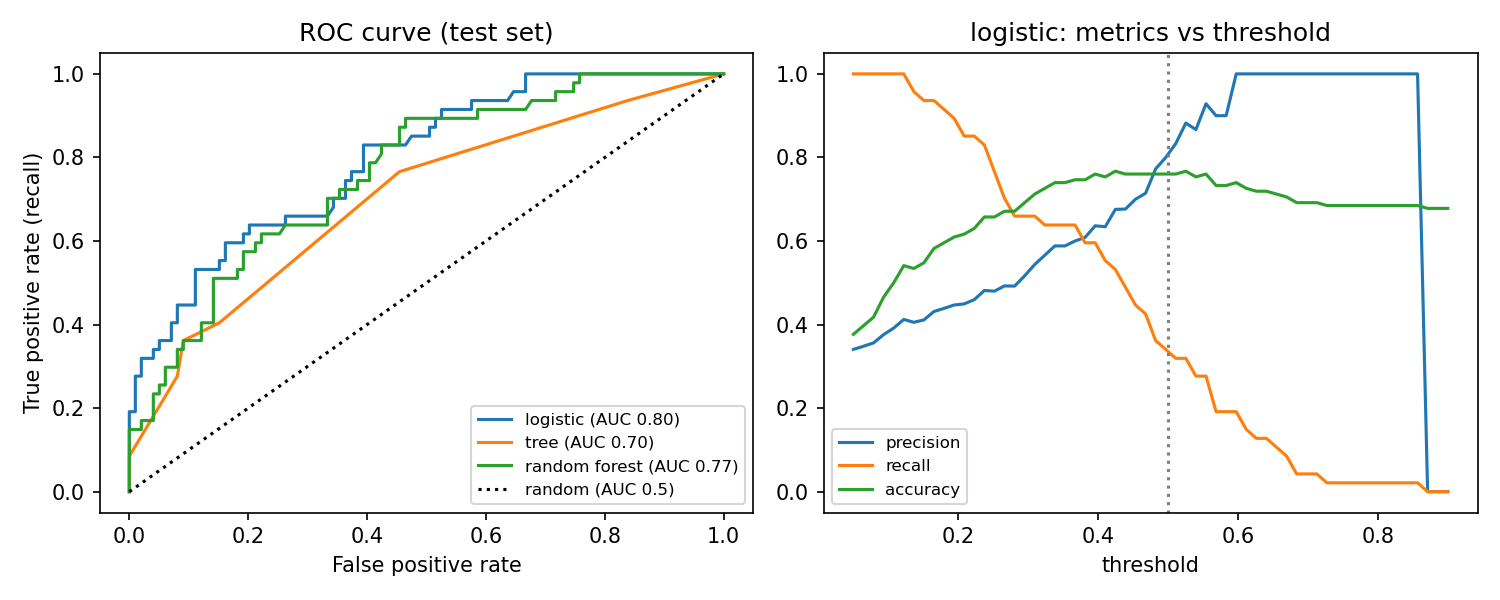
\includegraphics[width=\linewidth]{fig/clf_roc.png}
\end{center}
\begin{itemize}
\item \textbf{ROC 곡선} (왼쪽): 임계값을 1에서 0으로 내리며 (FPR, TPR)을 찍은 것. 왼쪽 위로 붙을수록 좋은 모델, 대각선은 동전 던지기.
\item \textbf{오른쪽}: 임계값에 따른 세 지표. 0.5 근처에서 정확도는 거의 평평하지만 recall은 급하게 떨어집니다.
\end{itemize}
\aside{※ 통계 연결: 임계값 선택은 가설검정의 $\alpha$ 선택과 같은 구조입니다. FP = Type I error, FN = Type II error, recall = power [흐름 11.4].}

\begin{qbox}
9. 임계값을 0으로 하면 confusion matrix는 어떻게 되나? recall과 precision은?
\end{qbox}

%=================================================
\section{Step 8. 다른 모델과 교차검증}
\begin{goalbox}{목표 \quad ⑨}
결정트리, 랜덤포레스트와 비교하되, test 한 번이 아니라 \textbf{5번 나눠서} 공정하게 비교한다.
\end{goalbox}

\subsection{교차검증 (cross-validation)}
582행을 5조각으로 나누고, 한 조각씩 돌아가며 평가용으로 씁니다. 5개 점수의 평균과 흩어짐을 봅니다.
\begin{center}\small
\begin{tabular}{@{}c c c c c c@{}}
\toprule
 & 조각 1 & 조각 2 & 조각 3 & 조각 4 & 조각 5 \\
\midrule
1회 & \textbf{평가} & 학습 & 학습 & 학습 & 학습 \\
2회 & 학습 & \textbf{평가} & 학습 & 학습 & 학습 \\
$\vdots$ & & & $\ddots$ & & \\
5회 & 학습 & 학습 & 학습 & 학습 & \textbf{평가} \\
\bottomrule
\end{tabular}
\end{center}

\begin{codebox}
pre\_tree = ColumnTransformer([("cat", OneHotEncoder(drop="first"), cat)], remainder="passthrough")\\
tree\ \ \ = Pipeline([("pre", pre\_tree), ("clf", DecisionTreeClassifier(max\_depth=\_\_\_, min\_samples\_leaf=20, random\_state=0))])\\
forest = Pipeline([("pre", pre\_tree), ("clf", RandomForestClassifier(n\_estimators=300, min\_samples\_leaf=10, random\_state=0))])\\
cv = StratifiedKFold(\_\_\_, shuffle=True, random\_state=0)\\
for name, m in [("logit", logit), ("tree", tree), ("forest", forest)]:\\
\ \ \ \ s = cross\_val\_score(m, \_\_\_, \_\_\_, cv=cv, scoring="roc\_auc") \hfill \# 전체 X, y\\
\ \ \ \ print(name, s.round(3), "mean", s.mean().round(3))
\end{codebox}
\begin{outbox}
logit\ \ [0.781 0.816 0.659 0.783 0.749] mean 0.758\\
tree\ \ \ [0.715 0.773 0.656 0.738 0.685] mean 0.714\\
forest [0.783 0.81\ \ 0.671 0.78\ \ 0.769] mean 0.763
\end{outbox}

\begin{howbox}
\begin{enumerate}
\item 모델마다 5번 학습·평가 = 총 15번 학습. 매번 파이프라인 전체(전처리 포함)를 그 회차의 학습 조각으로만 \code{fit}합니다 (leakage 없음).
\item 같은 \code{cv} 객체를 쓰므로 세 모델이 \emph{같은 조각}으로 비교됩니다.
\item 조각 3에서 세 모델 모두 낮음 (0.66 근처): 그 조각이 어려운 것이지 모델 탓이 아닙니다. 점수가 0.66–0.82로 흔들린다는 것 자체가 중요한 정보입니다.
\item logistic 0.758 vs forest 0.763: 차이(0.005)가 회차 간 흔들림(SD 약 0.05)보다 훨씬 작습니다. \textbf{사실상 같은 성능}이고, 해석이 쉬운 logistic을 고릅니다.
\end{enumerate}
\end{howbox}
\aside{※ 트리 모형은 표준화가 필요 없어서 (\code{remainder="passthrough"}) 숫자 열을 그대로 넘깁니다. 트리는 값의 \emph{순서}만 보고 분할하기 때문입니다 [알고 6, 7].}\\
\aside{※ 통계 연결: ``두 모델의 차이가 우연 범위인가''는 가설검정의 질문입니다. 5개 점수의 차이에 paired $t$-test를 할 수도 있습니다 [흐름 12 ⑥].}

\begin{qbox}
10. test set 점수(logit 0.796)와 교차검증 평균(0.758)이 다른 이유는?
\end{qbox}

%=================================================
\section{Step 9. 해석: 계수와 중요도}
\begin{goalbox}{목표 \quad ⑩}
모델이 \textbf{무엇을 보고} 예측하는지 확인한다.
\end{goalbox}

\begin{codebox}
names = logit.named\_steps["pre"].get\_feature\_names\_out()\\
coef\ \ = logit.named\_steps["clf"].coef\_[0]\\
print(pd.DataFrame(\{"feature": names, "coef": coef.round(3),\\
\ \ \ \ \ \ \ \ \ \ \ \ \ \ \ \ \ \ \ "odds\_ratio": np.\_\_\_(coef).round(2)\}))\\[3pt]
pi = permutation\_importance(logit, X\_test, y\_test, scoring="roc\_auc",\\
\ \ \ \ \ \ \ \ \ \ \ \ \ \ \ \ \ \ \ \ \ \ \ \ \ \ \ n\_repeats=30, random\_state=0)\\
imp = pd.Series(pi.importances\_mean, index=X.columns)\\
print(imp.round(3).sort\_values(ascending=False))
\end{codebox}
\begin{outbox}
\ \ \ \ \ \ \ \ \ \ \ \ \ \ \ \ \ \ \ \ \ feature\ \ \ coef\ \ odds\_ratio\\
0\ \ \ \ \ \ \ \ \ \ \ \ \ \ cat\_\_gender\_M\ \ 0.297\ \ \ \ \ \ \ \ 1.35\\
1\ \ cat\_\_department\_Marketing -1.256\ \ \ \ \ \ \ \ 0.28\\
2\ \ \ \ \ \ \ \ \ cat\_\_degree\_Master\ \ 0.175\ \ \ \ \ \ \ \ 1.19\\
3\ \ \ \ \ \ \ \ \ \ \ \ cat\_\_degree\_PhD\ \ 0.298\ \ \ \ \ \ \ \ 1.35\\
4\ \ \ \ \ \ \ \ \ \ \ \ num\_\_test\_score\ \ 0.627\ \ \ \ \ \ \ \ 1.87\\
5\ \ \ \ \ \ num\_\_years\_experience\ \ 0.351\ \ \ \ \ \ \ \ 1.42\\[3pt]
department 0.106 \quad test\_score 0.095 \quad years\_experience 0.032 \quad degree 0.016 \quad gender 0.010
\end{outbox}

\begin{howbox}
\begin{enumerate}
\item \textbf{Odds ratio}: Marketing이면 합격 odds가 0.28배, 점수가 1 SD (약 11.7점) 높으면 1.87배, 남성이면 1.35배 [응용 7.3].
\item \textbf{Permutation importance}: 한 열의 값을 test 안에서 무작위로 섞었을 때 AUC가 얼마나 떨어지나. 부서를 섞으면 0.106 하락, 성별은 0.010.
\item 계수는 ``한 단위 변할 때의 효과'', permutation은 ``그 정보가 없으면 예측이 얼마나 나빠지나''. 성별 계수가 0이 아닌데 중요도가 작은 이유: 성별 정보의 상당 부분이 부서에 이미 들어 있기 때문입니다 (성별 $\times$ 부서 $\chi^2=132$ [흐름 12 ⑧]).
\end{enumerate}
\end{howbox}
\aside{※ 응용 책의 statsmodels logit은 남성 odds ratio 1.60이었습니다. 여기서 1.35인 이유: (1) train 436명만 썼고, (2) sklearn의 \code{LogisticRegression}은 기본으로 L2 규제(\code{C=1})를 걸어 계수를 0 쪽으로 줄입니다. 규제 = Bayesian prior [응용 8.6]. 해석과 검정이 목적이면 statsmodels, 예측이 목적이면 sklearn을 씁니다.}

\begin{qbox}
11. 섞기(permutation)를 train이 아니라 test에서 하는 이유는?
\end{qbox}

%=================================================
\section{Step 10. 공정성 감사 (fairness audit)}
\begin{goalbox}{목표 \quad ⑪}
모델이 \textbf{성별에 따라 다르게 틀리는지} 확인한다. 이 워크북의 핵심 단계.
\end{goalbox}

\subsection{그룹별로 혼동행렬 쪼개기}
\begin{codebox}
def group\_report(p, thr=0.5):\\
\ \ \ \ t = X\_test.copy()\\
\ \ \ \ t["y"] = y\_test.values\\
\ \ \ \ t["y\_hat"] = (p >= thr).astype(int)\\
\ \ \ \ return t.groupby(\_\_\_).apply(lambda g: pd.Series(\{\\
\ \ \ \ \ \ \ \ "n": len(g),\\
\ \ \ \ \ \ \ \ "actual\_rate": g["y"].mean(),\\
\ \ \ \ \ \ \ \ "selection\_rate": g["y\_hat"].mean(),\\
\ \ \ \ \ \ \ \ "TPR": g.loc[g["y"] == \_\_\_, "y\_hat"].mean(), \hfill \# 실제 합격자 중 합격 예측\\
\ \ \ \ \ \ \ \ "FPR": g.loc[g["y"] == \_\_\_, "y\_hat"].mean(), \hfill \# 실제 불합격자 중 합격 예측\\
\ \ \ \ \}), include\_groups=False).round(3)\\
print(group\_report(p))
\end{codebox}
\begin{outbox}
\ \ \ \ \ \ \ \ \ \ n\ \ actual\_rate\ \ selection\_rate\ \ \ \ TPR\ \ \ \ FPR\\
F\ \ \ \ 77.0\ \ \ \ \ \ \ \ 0.182\ \ \ \ \ \ \ \ \ \ \ 0.026\ \ 0.071\ \ 0.016\\
M\ \ \ \ 69.0\ \ \ \ \ \ \ \ 0.478\ \ \ \ \ \ \ \ \ \ \ 0.261\ \ 0.455\ \ 0.083
\end{outbox}

\begin{howbox}
\begin{enumerate}
\item test의 여성 77명 중 실제 합격자 14명 (18.2\%), 남성 69명 중 33명 (47.8\%).
\item 모델이 합격이라고 예측한 사람: 여성 2명 (2.6\%), 남성 18명 (26.1\%).
\item \textbf{TPR (재현율)}: 실제 합격한 여성 14명 중 모델이 찾아낸 사람은 \textbf{1명} (0.071). 실제 합격한 남성 33명 중에서는 15명 (0.455).
\item 즉 \emph{똑같이 합격할 사람}이라도, 여성이면 모델에게 거의 발견되지 않습니다. 이것이 \term{equal opportunity} (그룹 간 TPR이 같아야 한다) 위반입니다 [응용 9.1].
\end{enumerate}
\end{howbox}

\subsection{성별을 빼면 해결될까? (fairness through unawareness)}
\begin{codebox}
pre2 = ColumnTransformer([("cat", OneHotEncoder(drop="first"), [\_\_\_]),\\
\ \ \ \ \ \ \ \ \ \ \ \ \ \ \ \ \ \ \ \ \ \ \ \ \ ("num", StandardScaler(), num)])\\
logit2 = Pipeline([("pre", pre2), ("clf", LogisticRegression(max\_iter=1000))])\\
logit2.fit(X\_train, y\_train)\\
p2 = logit2.predict\_proba(X\_test)[:, 1]\\
print(group\_report(p2))
\end{codebox}
\begin{outbox}
\ \ \ \ \ \ \ \ \ \ n\ \ actual\_rate\ \ selection\_rate\ \ \ \ TPR\ \ \ \ FPR\\
F\ \ \ \ 77.0\ \ \ \ \ \ \ \ 0.182\ \ \ \ \ \ \ \ \ \ \ 0.091\ \ 0.071\ \ 0.095\\
M\ \ \ \ 69.0\ \ \ \ \ \ \ \ 0.478\ \ \ \ \ \ \ \ \ \ \ 0.246\ \ 0.424\ \ 0.083
\end{outbox}
\begin{howbox}
\begin{enumerate}
\item 성별 열을 빼도 여성 TPR은 \textbf{그대로 0.071}, 남성은 0.424. 격차가 거의 안 줄었습니다.
\item 이유: \textbf{proxy (대리) 변수}. 여성의 68\%가 Marketing에 지원했고 Marketing은 합격률이 낮습니다. 모델은 ``Marketing''을 통해 성별 정보를 간접적으로 씁니다.
\item 오히려 여성 FPR이 0.016 $\to$ 0.095로 올라, 여성에게서 ``잘못 합격''이 늘었습니다. 성별을 빼는 것만으로는 공정해지지 않습니다.
\end{enumerate}
\end{howbox}

\subsection{반사실 테스트: 성별만 바꾸면?}
\begin{codebox}
X\_flip = X\_test.copy()\\
X\_flip["gender"] = X\_flip["gender"].map(\{"M": \_\_\_, "F": \_\_\_\})\\
p\_flip = logit.predict\_proba(X\_flip)[:, 1]\\
print("결정이 바뀐 사람:", ((p\_flip >= 0.5) != (p >= 0.5)).sum(), "/", len(X\_test))
\end{codebox}
\begin{outbox}
결정이 바뀐 사람: 14 / 146
\end{outbox}
\aside{※ 다른 조건은 모두 같고 성별만 바꿨는데 146명 중 14명(약 10\%)의 합불이 뒤집혔습니다. 평균적으로 여성 $\to$ 남성으로 바꾸면 합격 확률 +4.6\%p, 남성 $\to$ 여성이면 $-5.9$\%p. 응용 책 \code{assign(gender="M")} 계산과 같은 반사실 논리입니다 [응용 7장 pandas 코드].}

\begin{qbox}
12. 여성 TPR 0.071은 실제 합격 여성 14명에 기반한다. 이 숫자를 발표할 때 함께 말해야 할 주의점은?
\end{qbox}

%=================================================
\section{정리와 발표}
\begin{goalbox}{목표 \quad ⑫}
분류 결과를 ``bias in hiring'' 질문에 대한 답으로 바꾼다.
\end{goalbox}

\subsection{이번 실습으로 알게 된 것}
\begin{center}\small
\begin{tabular}{@{}l p{11cm}@{}}
\toprule
단계 & 결과 \\
\midrule
기준선 & 전원 불합격 예측으로도 정확도 0.678 $\to$ 정확도만으로는 판단 불가 \\
logistic & 정확도 0.760, AUC 0.796 (CV 0.758). 합격자를 34\%만 찾음 \\
모델 비교 & tree 0.714, forest 0.763: logistic과 사실상 같음 $\to$ 해석 쉬운 logistic 선택 \\
중요 특성 & 부서 $>$ 점수 $>$ 경력 $>$ 학위 $>$ 성별 (permutation) \\
공정성 & 실제 합격 여성 중 1/14만 발견 (TPR 0.07 vs 남성 0.46) \\
성별 제거 & 격차 유지 (부서가 proxy) \\
반사실 & 성별만 바꾸면 10\%의 결정이 뒤집힘 \\
\bottomrule
\end{tabular}
\end{center}

\subsection{발표용 문장 (예시)}
\begin{goalbox}{이렇게 말하면 된다}
``과거 채용 데이터로 합격 예측 모델을 학습시키면 정확도 76\%, AUC 0.80의 모델이 나온다. 그러나 이 모델은 실제로 합격한 여성 14명 중 1명만 합격으로 예측했고, 남성은 33명 중 15명을 찾았다. 성별 변수를 제거해도 지원 부서가 성별의 대리 변수로 작동해 격차가 유지된다. 다른 조건은 같고 성별만 바꿔도 약 10\%의 결정이 뒤집힌다. 즉, 이 데이터로 자동화된 채용 시스템을 만들면 과거의 성별 격차를 그대로 재생산할 위험이 크다. 단, test의 여성 합격자가 14명뿐이라 수치의 불확실성이 크므로, 통계 분석(응용 책 6–8장)의 결론과 함께 제시한다.''
\end{goalbox}

\subsection{다음에 해 볼 것}
\begin{itemize}
\item 임계값을 그룹별로 달리해서 TPR을 맞추기 (post-processing). 공정성은 좋아지지만 ``성별에 따라 다른 기준''이라는 법적·윤리적 문제가 생깁니다 [응용 9.1 impossibility].
\item 부서별로 따로 모델 만들기: Engineering 안에서의 격차만 보기 (응용 책 interaction과 비교).
\item 공정성 지표에 bootstrap 신뢰구간 붙이기 [흐름 9.2]: 14명짜리 TPR이 얼마나 흔들리는지.
\end{itemize}

%=================================================
\section{확인 질문 답과 빈칸 정답}
\subsection{확인 질문}
\textbf{1.} 회귀 (정답이 숫자). \quad \textbf{2.} 아닙니다. 정확도는 과거 결정을 얼마나 잘 따라 하느냐이고, 과거 결정이 편향이면 정확한 모델도 편향입니다 (11장).

\textbf{3.} 네. \code{drop}은 지정한 열을 \emph{빼고} 나머지를 남깁니다. 열이 많을 때 편합니다.

\textbf{4.} 우연히 test에 합격자가 너무 적거나 많게 들어갈 수 있습니다. 합격자 5\%(582명 중 약 29명)면 test 146명에 합격자가 3명만 들어갈 수도 있어서, recall 같은 지표가 몇 명에 좌우됩니다.

\textbf{5.} 95\%. 그래서 불균형 데이터에서는 정확도 대신 recall, precision, AUC를 봅니다.

\textbf{6.} ``점수 1점당 log-odds 변화''. 표준화하면 ``1 SD(약 11.7점)당''이 됩니다. 예측 확률은 같지만 (규제가 없다면) 계수의 숫자만 바뀝니다.

\textbf{7.} 이 지원자는 Engineering (기준 범주)이라 \code{department\_Marketing} = 0이고, $-1.256\times0=0$입니다.

\textbf{8.} 1차 통과는 ``좋은 사람을 놓치지 않기''가 중요하므로 \textbf{recall}. 최종 합격 결정이라면 precision이 더 중요할 수 있습니다.

\textbf{9.} 모두 1로 예측하므로 TN = FN = 0, \code{[0 99 0 47]}. recall = 1, precision = 47/146 = 0.322 (합격률).

\textbf{10.} test 146명은 한 번의 무작위 분할 결과라 운이 섞입니다. CV는 5번의 평균이라 더 안정적인 추정입니다. 이번 test 분할은 쉬운 편이었습니다.

\textbf{11.} 모델이 본 적 없는 데이터에서 ``그 정보가 예측에 얼마나 필요한가''를 재야 하기 때문입니다. train에서 재면 외운 패턴까지 중요하다고 나옵니다.

\textbf{12.} 14명 중 1명이라 한두 명만 달라져도 TPR이 크게 바뀝니다 (1/14 = 0.07, 3/14 = 0.21). 표본 크기를 함께 말하고, 가능하면 교차검증이나 bootstrap으로 구간을 제시합니다.

\subsection{빈칸 정답}
\begin{center}\small
\begin{tabular}{@{}l l@{}}
\toprule
Step & 빈칸 \\
\midrule
1 & \code{dropna}, \code{cat + num}, \code{"hired"} \\
2 & \code{0.25}, \code{y} \\
3 & \code{"most\_frequent"} \\
4 & \code{OneHotEncoder}, \code{StandardScaler} \\
5 & \code{fit}, \code{predict\_proba}, \code{0.5} \\
6 & \code{tp + tn}, \code{tp + fp}, \code{tp + fn}, \code{p} \\
7 & \code{thr} \\
8 & \code{3}, \code{5}, \code{X}, \code{y} \\
9 & \code{exp} \\
10 & \code{"gender"}, \code{1}, \code{0}, \code{"department", "degree"}, \code{"F"}, \code{"M"} \\
\bottomrule
\end{tabular}
\end{center}
\aside{※ 전체 정답 코드와 출력은 \code{classification\_solution.ipynb}에 있습니다.}

\end{document}
